\section{3-Omniwheel Simulation [55 pts]}
\begin{enumerate}[(a)]
    \item Derive the equation of motion (as we did for the 4W during the lectures) for the omnidirectional wheeled robot with three wheels shown in see Figure~\ref{fig:3omni} [25 pts]
    
    \item Create a simulation for this robot with MATLAB or Python (you want to obtain $x,y,\theta$ for your simulation, you can obtain $\dot{x},\dot{y},\dot{\theta}$ as function of the wheels speeds by inverting the relationship obtained in (a)). Use $r=10$ cm and $l=25$ cm.
    \begin{enumerate}[I.]
        \item Apply rotation inputs (wheel rotation speeds) of $u_1=-2$ rad/s, $u_2=1.0$ rad/s and $u_3=1.0$ rad/s to the wheels and plot the true robot motion $(x,y,\theta)$ for 30 seconds. Plot the variables against time, and also a top view of the trajectory ($x$ vs $y$).
        \item Design control signals $(u_1,u_2,u_3)$ that will allow the robot to move in the following paths (simulation time is up to you, we recommend using at least 30 seconds):\begin{enumerate} [1)]
            \item a straight line with a slope of 60 degrees
            \item turn in a 2-meter diameter circle.
            \end{enumerate} 
        Use your simulation to confirm the obtained control signals by plotting the two cases, plot the variables against time, and also a top view of the trajectory ($x$ vs $y$). 
    \end{enumerate} 
\end{enumerate}
\begin{figure}[h!]
    \centering
    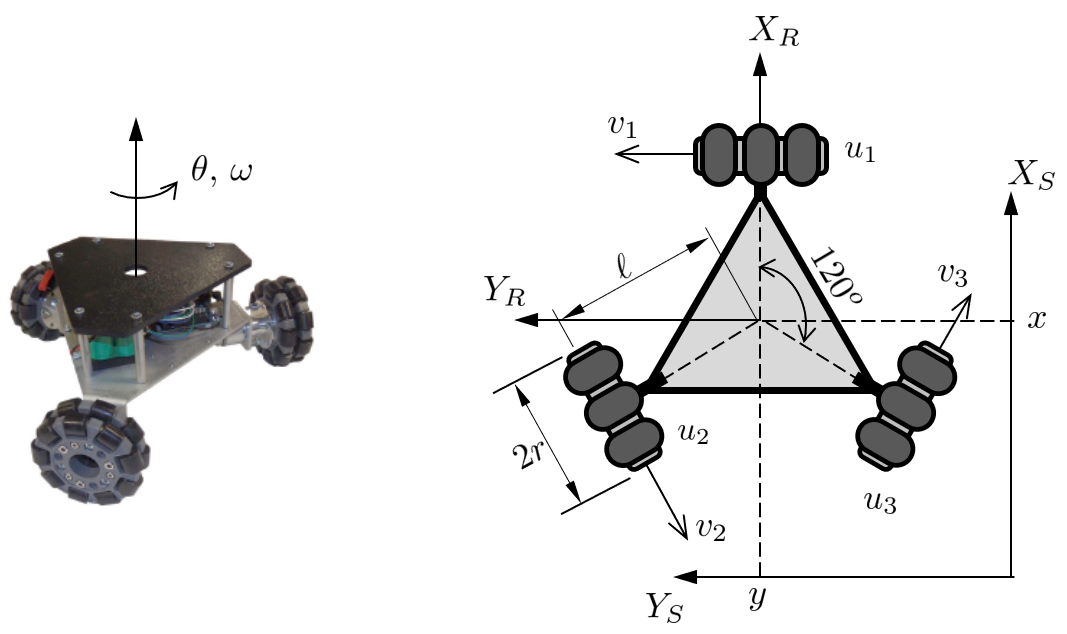
\includegraphics[width=0.7\textwidth]{img/omni.png}
    \caption{3W omnidirectional robot}
    \label{fig:3omni}
\end{figure}